\section{Demonstration}

The CPR demo is provided as a Git repository and associated Docker image that enable the examples to be run on any Linux, macOS, or Windows-based system with Git, Docker, and GNU Make installed.  Each example uses the CPR toolkit to record OS-level provenance information from a run of different computational workflow, to load a Blazegraph instance with the resulting CPR traces, and to produce a set of reports and visualizations via SPARQL queries.
 
A Makefile in the top directory of the demo repository provides targets for pulling the Docker image from Dockerhub (\commandtext{pull-image}), building the Docker image locally (\commandtext{build-image}), for running the examples (\commandtext{run-examples}), and for deleting all of the reports, visualizations, and other artifacts generated for each example (\commandtext{clean-examples}). Because the expected results are included in the repository, successful reproduction of the example products is demonstrated by issuing the commands \commandtext{make clean-examples} and \commandtext{make run-examples} and confirming that \commandtext{git diff} reports no differences.

\begin{figure}[h!]
    
    \begin{subfigure}[b]{1.0\linewidth}
        \begin{lstlisting}
#!/bin/bash
cat inputs/i1.txt inputs/i2.txt > temp/t12.txt
cat inputs/i1.txt inputs/i2.txt inputs/i3.txt > temp/t123.txt
cat inputs/i4.txt > temp/t4.txt
cat temp/t12.txt > outputs/o12.txt
cat temp/t123.txt temp/t4.txt > outputs/o1234.txt
cat temp/t4.txt > outputs/o4.txt
        \end{lstlisting}
        \setlength{\abovecaptionskip}{-2pt}
        \setlength{\belowcaptionskip}{15pt}
        \caption{Workflow script.}
    \end{subfigure}

    \begin{subfigure}[b]{1.0\linewidth}

        \begin{subfigure}[b]{0.25\linewidth}
            \begin{lstlisting}
roles:
  os:
    - /etc
    - /lib
    - /usr/lib
  sw:
    - /usr/bin
  in:
    - ./inputs
  out:
    - ./outputs
  tmp:
    - ./temp
            \end{lstlisting}
            \setlength{\abovecaptionskip}{-2pt}
            \setlength{\belowcaptionskip}{15pt}
            \caption{Run profile.}
        \end{subfigure}

        \begin{subfigure}[b]{0.69\linewidth}
            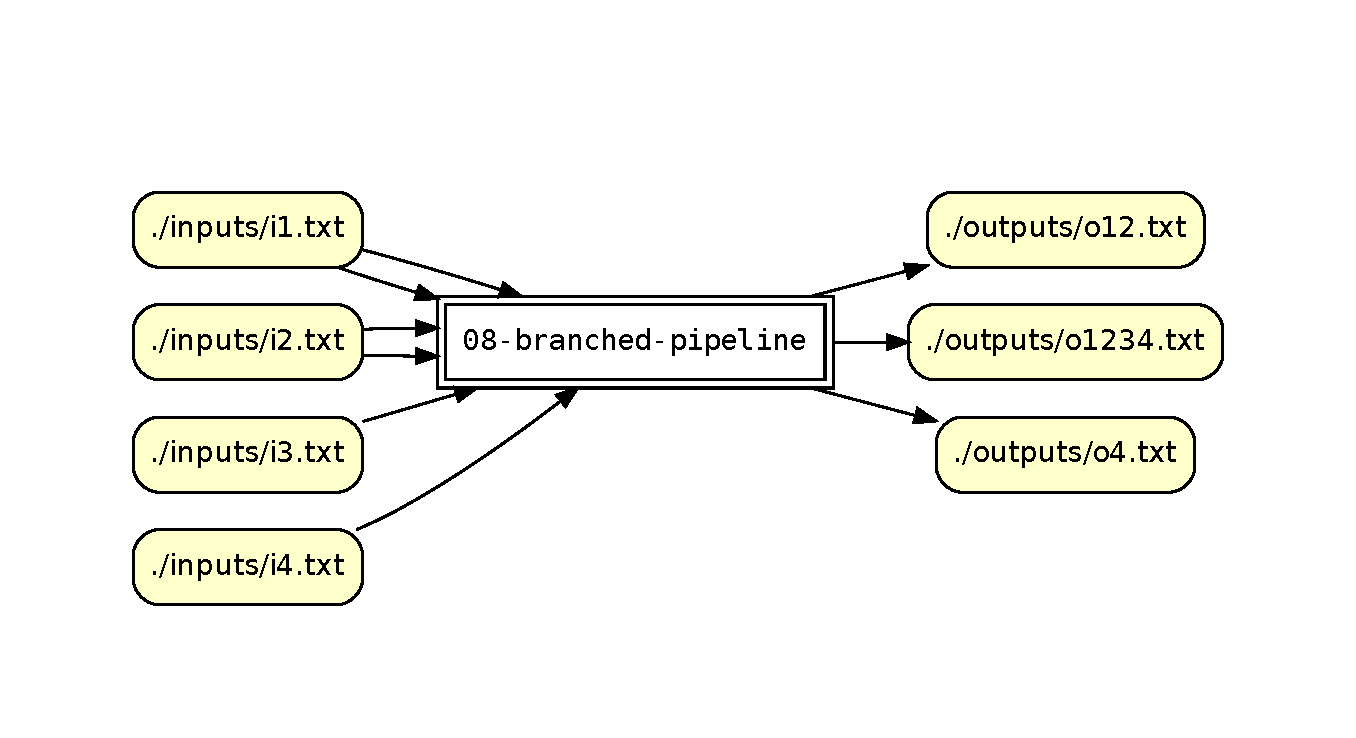
\includegraphics[width=\linewidth]{cpr_run_inputs_outputs.pdf}
            \setlength{\abovecaptionskip}{-5pt}
            \setlength{\belowcaptionskip}{15pt}
            \caption{Visualization of inputs and outputs of the run as a whole.}
        \end{subfigure}

    \end{subfigure}

    \begin{subfigure}[b]{1.0\linewidth}
        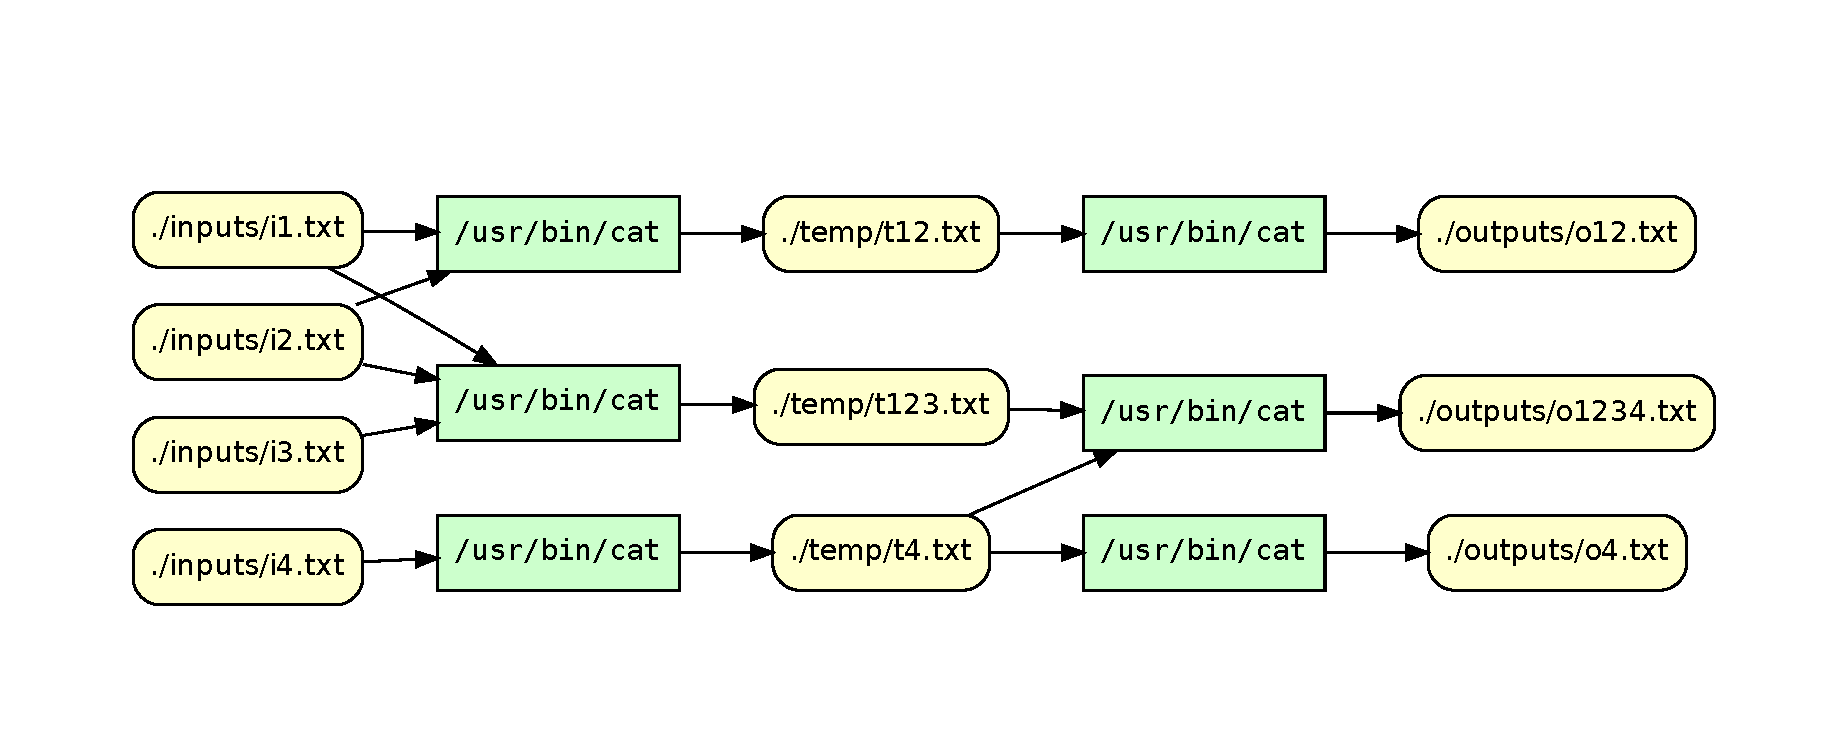
\includegraphics[width=\linewidth]{cpr_processes_and_data_files.pdf}
        \setlength{\abovecaptionskip}{-5pt}
        \caption{Flow of data files through processes comprising the run.}
    \end{subfigure}
    
    \label{fig:cpr-example}
\end{figure}
 

The examples range from the trivial and domain-independent, to relatively complex and domain-specific.  An example of minimal complexity that still demonstrates key capabalities of CPR is illustrated in Figure \ref{fig:cpr-example}. A simple bash script invokes the \commandtext{cat} command six times on different combinations of three input files to produce three intermediate files, and three final output files (each a distinct concatenation of the three input files).  
